% !TEX root = ../presentation.tex

\begin{frame}{Main Claim}
	\begin{block}{One-sentence takeaway}
		State the thesis result in one sentence before showing supporting details.
	\end{block}

	\begin{itemize}
		\item Keep slide text short.
		\item Move details to backup slides or the written thesis.
		\item Cite sources when needed, e.g. \parencite{lamport1994latex}.
	\end{itemize}
\end{frame}

\begin{frame}{Figure and Table}
	\begin{columns}[T,onlytextwidth]
		\column{0.52\textwidth}
		\centering
		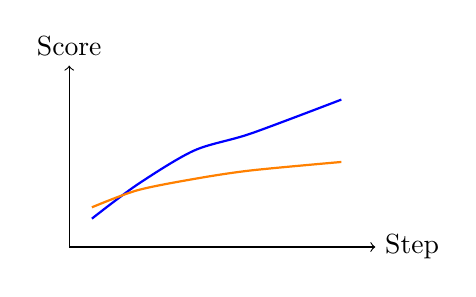
\begin{tikzpicture}[scale=0.72]
			\draw[->] (0,0) -- (5.4,0) node[right] {Step};
			\draw[->] (0,0) -- (0,3.2) node[above] {Score};
			\draw[thick,blue] plot[smooth] coordinates {(0.4,0.5) (1.2,1.1) (2.2,1.7) (3.2,2.0) (4.8,2.6)};
			\draw[thick,orange] plot[smooth] coordinates {(0.4,0.7) (1.2,1.0) (2.2,1.2) (3.2,1.35) (4.8,1.5)};
		\end{tikzpicture}

		\column{0.43\textwidth}
		\centering
		\begin{tabular}{lrr}
			\toprule
			Method & A & B \\
			\midrule
			Base & 71 & 12 \\
			Ours & 83 & 11 \\
			\bottomrule
		\end{tabular}
	\end{columns}
\end{frame}
